%------------------------------------- CONFIGURAÇÕES DE CAPA --------------------------------------
\begin{titlepage}
	
	% Capa Principal
	\begin{center}
		\Huge{UNIVERSIDADE DE SÃO PAULO}\\
		\vspace{0.02\textheight}
		\huge{ESCOLA DE ENGENHARIA DE SÃO CARLOS}\\
		\vspace{0.01\textheight}
		\huge{DEPARTAMENTO DE ENGENHARIA ELÉTRICA}\\
		\vspace{0.2\textheight}
		\huge{\textbf{Desenvolvimento de algoritmo de visão para VANTS sobre Linux Embarcado}}
		\vspace{0.2\textheight}
	\end{center}
		
		\large
		{
			\begin{flushleft}
			\Large{ \textbf{Autor}: \hspace{1cm} Nícolas dos Santos Rosa}\\
			\Large{ \textbf{Orientador}: \hspace{0.3cm} Prof. Dr. Evandro Luís Linhari Rodrigues }\\
			\end{flushleft}
	
			\begin{center}
				\vspace{0.09\textheight}
				\Large{São Carlos}\\
				\Large{2015}
			\end{center}
		}
	
\end{titlepage}


%------------------------------------- INSERÇÃO PÁGINA EM BRANCO ------------------------------------
\cleardoublepage

%------------------------------------- FOLHA DE ROSTO  ----------------------------------------------
%\vspace{0.01\textheight} 
	\begin{center}
	\vspace{-0.06\textheight}
	%\thispagestyle{empty}
		\Large{\textbf{Nícolas dos Santos Rosa}}\\
		\vspace{0.15\textheight}
		\Huge{\textbf{Desenvolvimento de algoritmo de visão para VANTS sobre Linux Embarcado}} 
		\vspace{0.08\textheight}
	\end{center}
		
		\large
		{
			\begin{flushright}
			\Large{Trabalho de Conclusão de Curso apresentado} \hspace{1cm}\\
			\Large{à Escola de Engenharia de São Carlos, da}\\
			\Large{Universidade de São Paulo}\\
			\vspace{0.05\textheight}
			\Large{Curso de Engenharia Elétrica}\\
			\vspace{0.05\textheight}
			\Large{ORIENTADOR: Prof. Evandro Luís Linhari Rodrigues}\\
			\end{flushright}
	
			\begin{center}
				\vspace{0.15\textheight}
				\Large{São Carlos}\\
				\Large{2015}
			\end{center}
		}



%------------------------------------- FICHA CATALOGRÁFICA ------------------------------------------
\newpage

Página com a ficha catalográfica (em página par).

%ficha catalografica no verso
%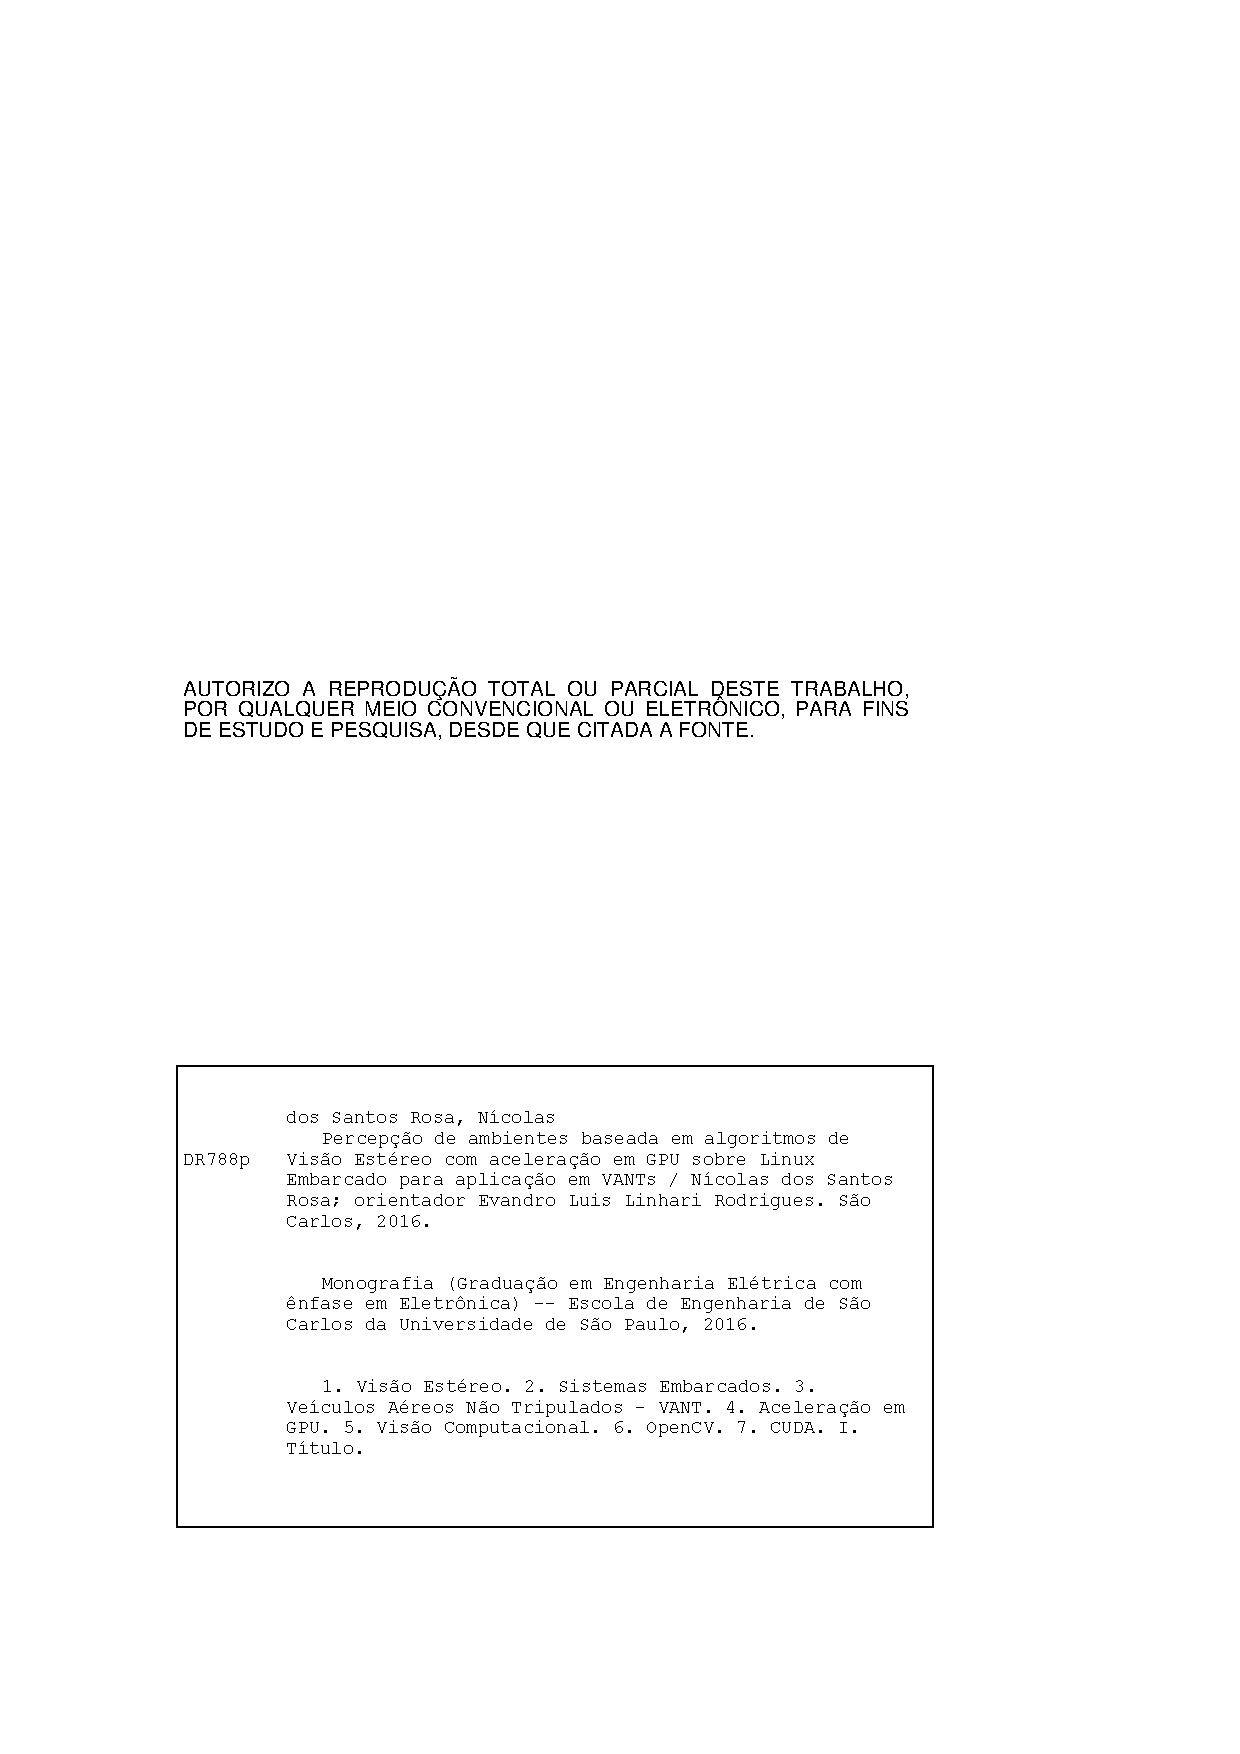
\includepdf{./Resources/ficha_catalografica.pdf}

%------------------------------------- Folha de aprovação--------------------------------------------
\newpage

página com a folha de aprovação (página ímpar). \cleardoublepage

\begin{comment}
\begin{figure}[H]
	\centering
	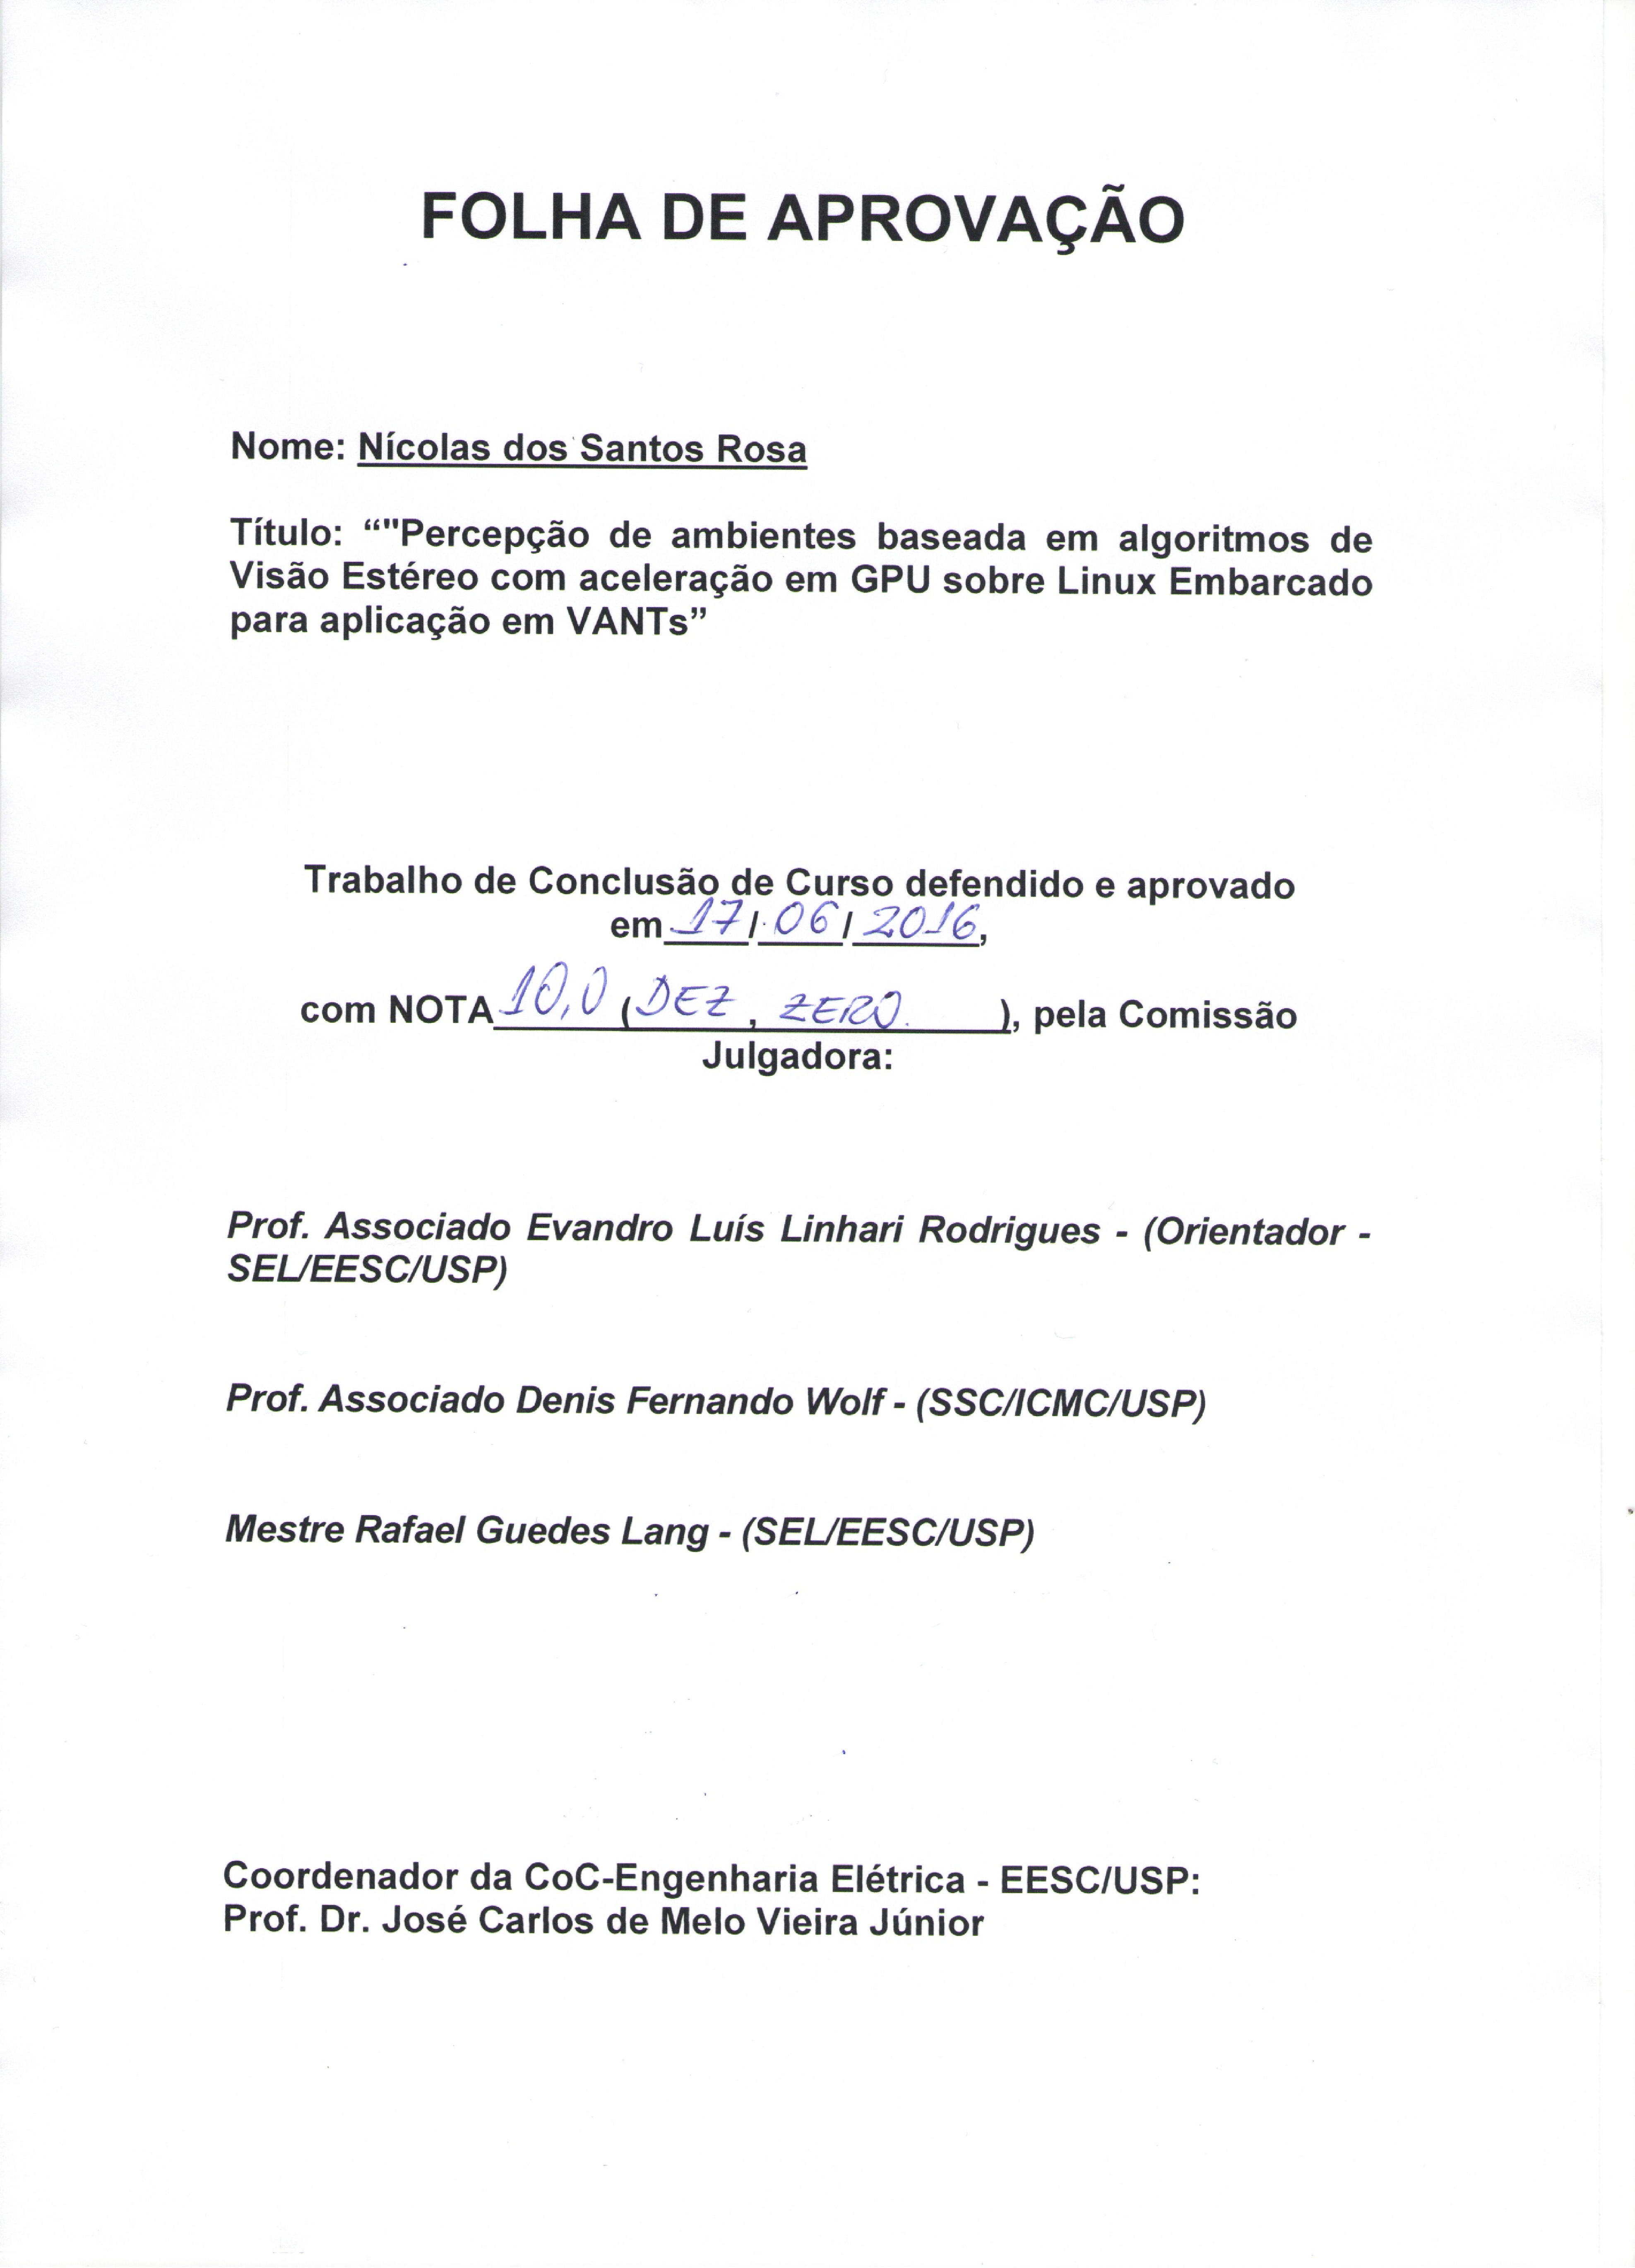
\includegraphics[scale=0.3]{./Resources/aprovacao.jpg}
	\caption{Fluxo de comunicação entre os principais componentes.}
	\label{Aprovacao}
\end{figure}
\cleardoublepage
\end{comment}
%------------------------------------- Dedicatória --------------------------------------------------
\
\vspace{0.11\textheight} 
\begin{center}
\textbf{\Huge{Dedicatória}}
\end{center}
\vspace{0.05\textheight}	
		
Este trabalho de conclusão de curso é dedicado a minha mãe, meu pai, minha irmã, meus padrinhos e toda minha família.
		
\begin{flushright}
Nícolas dos Santos Rosa.
\end{flushright}

%------------------------------------- INSERÇÃO PÁGINA EM BRANCO ------------------------------------
\cleardoublepage

%------------------------------------- Agradecimentos -----------------------------------------------
\
\vspace{0.11\textheight} 

\begin{center}
\textbf{\Huge{Agradecimentos}}
\end{center}

\vspace{0.05\textheight}
			
Primeiramente, agradeço a Deus por propiciar saúde e felicidade a todos aqueles que me rodeiam.

À minha família: à minha Mãe, Valdenilce, pela ferranha dedicação em mostrar a mim e a minha irmã a importância da educação para nossa formação pessoal; ao meu pai, Francisco, por fazer o possível e o impossível para sustentar nossa família e por possibilitar condições para que me tornasse engenheiro; à minha irmã, Natália, pelo suporte e carinho e por ser a dupla perfeita para atazanar nossos pais; às minhas tias, Elisabeth, Vera Lúcia e Maria Regina, por serem minhas segundas mães, visto o tamanho do suporte, preocupação, e apreço dado. 

Ao meu orientador, Prof. Evandro Luís Linhari Rodrigues, pelo apoio para o desenvolvimento deste trabalho e por despertar meu interesse em sistemas embarcados, confirmando ainda mais minha paixão pelo meu curso.  

Aos meus orientadores de iniciação científica, Prof. Dr. Cláudio F. M. Toledo, Márcio S. Arantes, por introduzir-me ao âmbito da pesquisa acadêmica. Aos membros do SARLab: ao Prof. Dr. Samir Rawashdeh por ser o idealizador deste trabalho e por oferecer a oportunidade de desenvolvê-lo; a Benjamin Dale e a Miguel Rocha Jr., pelo companheirismo e por sempre estarem sempre de prontidão.

Aos meus amigos de curso, pelos ótimos momentos que vivemos juntos nestes anos, especialmente, Alexandre B. Moretti, Leonardo B. Farçoni, Plínio F. G. Bueno, Marília L. Dourado,  Jéssica B. da Vida, Pedro Arantes, Augusto Martins, Gustavo Oliveira, Aline Midori, Vitor Martins, Anderson M. Tsai, Victor Morini, João F. Corsini, Caio Martins e à todos os outros amigos. 

Aos membros do grupo extracurricular Warthog Robotics, por partilhar um interesse em comum e pelas incontáveis horas de dedicação gastas no laboratório.

Por fim, agradeço a todos os envolvidos no desenvolvimento deste trabalho.
		
\begin{flushright}
Nícolas dos Santos Rosa.
\end{flushright}


%------------------------------------- INSERÇÃO PÁGINA EM BRANCO ------------------------------------
\cleardoublepage

%------------------------------------- EPÍGRAFE -----------------------------------------------------
\
\vspace{0.76\textheight} 

\begin{flushright}

\textit{"O dinheiro faz homens ricos, o conhecimento faz homens }

\textit{sábios e a humildade faz grandes homens."}

Mahatma Gandhi

\textit{"You can't put a limit on anything. The more you dream, the farther you get."}

Michael Phelps

\textit{"Se eu vi mais longe, foi por estar sobre ombros de gigantes."}

Isaac Newton

\end{flushright}


%------------------------------------- INSERÇÃO PÁGINA EM BRANCO ------------------------------------
\cleardoublepage

%------------------------------------- RESUMO - PORTUGUÊS -------------------------------------------
\
\vspace{0.11\textheight} 

\begin{center}
\textbf{\Huge{Resumo}}
\end{center}

%Remover
%\textcolor{red}{\textbf{Dica:} Texto em um parágrafo apenas - deve conter "tudo" resumidamente (introdução, método(s), resultados e conclusões), de tal forma que seja possível compreender a proposta e o que foi alcançado;
%Palavras-chave: Logo abaixo do Resumo/Abstract.}

\vspace{0.05\textheight}

Rosa, Nícolas \textbf{Desenvolvimento de algoritmo de visão para VANTS sobre Linux Embarcado}. Trabalho de Conclusão de Curso -- Escola de Engenharia de São Carlos, Universidade de São Paulo, 2015.

Atualmente, veículos aéreos não tripulado (VANT) vem tornando-se um assunto recorrente no âmbito científico. Estes veículos, devido a sua mobilidade e inteligência artificial, vem sendo adaptados para a atuação em diferentes ambientes, desempenhando assim diversas atividades que vão desde
aplicações militares, agronômicas, espaciais, cinematográficas,entre outras.    
Entretanto, essa atuação só não é mais ampla devido a problemas relacionados ao reconhecimento do ambiente ao seu redor e detecção de objetos e obstáculos. Neste trabalho, estuda-se a utilização de visão estéreo em sistemas embarcados para reconhecimento de obstáculos que ameacem a locomoção do veículo autônomo. Por fim, será desenvolvido um algoritmo utilizando visão computacional que estime as distâncias de objetos próximos ao veículo móvel.

\vspace{0.05\textheight}
	
Palavras-Chave: Visão estéreo, Detecção de Obstáculos, Sistemas Embarcados, Veículos Aéreos Não Tripulado - VANT, Visão Computacional.

%------------------------------------- INSERÇÃO PÁGINA EM BRANCO ------------------------------------ 
\cleardoublepage

%------------------------------------- RESUMO - INGLÊS ----------------------------------------------
\
\vspace{0.11\textheight} 

\begin{center}
\textbf{\Huge{Abstract}}
\end{center}

\vspace{0.05\textheight}	
		
Currently, unmanned aerial vehicles (UAV) is becoming a recurring theme in the scientific realm. These vehicles, because of their mobility and artificial intelligence, have been adapted to perform in different environments, thus performing various activities ranging from
military applications, agronomic, spacial, cinematographic, among others.
However, this performance is not wider due to  problems related to the recognition of the surrounding environment and the detectition objects and obstacles. In this paper, it will be studied the use of stereoscopic vision in embedded systems to recognize obstacles that threaten the mobility of the autonomous vehicle. Finally, an algorithm using computer vision to estimate the distances of objects near the mobile vehicle will be developed.

\vspace{0.05\textheight}

Keywords: Stereo Vision, Obstacle Detection, Embedded Systems, Unmanned aerial Vehicle - UAV, Computational Vision.

%------------------------------------- INSERÇÃO PÁGINA EM BRANCO ------------------------------------
\cleardoublepage
%\thispagestyle{empty}
%\newpage
%------------------------------------- RESUMO -------------------------------------------------------

%------------------------------------- CONFIGURAÇÕES DOS ÍNDICES ------------------------------------
%\clearpage
%\thispagestyle{empty}
\listoffigures % Índice de Figuras

\listoftables % Índice de Tabelas

%------------------------------------- INSERÇÃO PÁGINA EM BRANCO ------------------------------------ 
\cleardoublepage

%------------------------------------- LISTA DE ABREVIATURAS ----------------------------------------
\
\vspace{0.11\textheight} 

\textbf{\Huge{Siglas}}

\vspace{0.05\textheight}
			
\begin{tabbing}
\hspace*{0.5cm}\=\hspace{2.5cm}\= \kill

% Lista de Abreviaturas
\> AAVC		\> \textit{Autonomous Aerial Vehicle Competition}									\\
\> AFRL		\> \textit{Air Force Research Laboratory} - Laboratório de pesquisas da Força Aérea Americana 				\\ 
\> ANAC		\> Agência Nacional de Aviação Civil 											\\
\> AUV		\> \textit{Autonomous Underwater Vehicle} - Veículo Submarinos Autônomo	 						\\
\> BBB		\> \textit{BeagleBone Black}	 											\\
\> BM		\> \textit{Block Matching} - Método Estéreo Local	 								\\
\> BMGPU	\> \textit{Block Matching with GPU Acceleration} - 									\\
\>		\> Método Estéreo Local com Aceleração de GPU										\\
\> CPU		\> \textit{Central Processing Unit} - Unidade central de Processamento							\\
\> CUDA		\> \textit{Compute Unified Device Architecture} - Plataforma de computação paralela					\\
\> DECEA	\> Departamento de Controle do Espaço Aéreo										\\
\> FAA	 	\> \textit{Federal Aviation Administration} - Administração Federal de Aviação						\\
\> FPGA  	\> \textit{Field-programmable gate array} - Arranjo de Portas Programável em Campo					\\
\> GUI 	 	\> \textit{Graphical User Interface} - Interface gráfica do usuário							\\
\> GPU 	 	\> \textit{Graphics Processing Unit} - Unidade de Processamento Gráfico							\\
\> GPGPU 	\> \textit{General Purpose Graphics Processing Unit} -  								\\
\>		\> Unidade de Processamento Gráfico de Propósito Geral									\\
\> GPS 	 	\> \textit{Global Positioning System} - Sistema de Posicionamento Global						\\
\> LMR 	 	\> Laboratório de Robótica Móvel											\\
\> MAVS  	\> \textit{Micro Air Vehicle} - Micro Veículo Aéreo									\\
\> MIT 	 	\> \textit{Massachusetts Institute of Technology}									\\
\> OACI  	\> Organização de Aviação Civil Internacional 										\\
\> RPA 	 	\> \textit{Remotely Piloted Aircraft} - Aeronave Remotamente Pilotada							\\
\> SGBM  	\> \textit{Semi-Global Block Matching}	- Método Estéreo Semi-global							\\
\> SLAM  	\> \textit{Simultaneous Localization and Mapping} - Localização e Mapeamento Simultâneo					\\
\> UAV/VANT 	\> \textit{Unmanned aerial vehicle} - Veículo Aéreo não tripulado 							\\

\end{tabbing}
\cleardoublepage
%------------------------------------- CONFIGURAÇÕES DOS ÍNDICES ------------------------------------ 
%\usepackage{fancyhdr}
\pagestyle{fancy}
\fancyhf{} % clear all header and footer fields
\fancyhead[RO, LE] {\thepage}

\fancypagestyle{plain}{\pagestyle{fancy}}

\tableofcontents % Índice Geral